\chapter{G\'eom\'etrie dans l'espace} \label{calcesp}
\minitoc

\fancyhead{} % efface les entêtes précédentes
\fancyhead[LE,RO]{\footnotesize \em \rightmark} % subsection en entête
\fancyhead[RE,LO]{\scriptsize \em Seconde} % classe et année en entête

    \fancyfoot{}
		\fancyfoot[RE]{\scriptsize \em \href{http://perpendiculaires.free.fr/}{http://perpendiculaires.free.fr/}}
		\fancyfoot[LO]{\scriptsize \em David ROBERT}
    \fancyfoot[LE,RO]{\textbf{\thepage}}

%\sautpage



\section{Perspective cavalière}

\subsection{Principe}
%\begin{tabular}{cc}
%\begin{minipage}[l]{0.725\linewidth}
 Dans ce chapitre, nous allons travailler sur des objets en trois dimensions qui seront représentés, la plupart du temps, sur des feuilles de papier qui, elles, n'ont que deux dimensions et sur lesquelles il faudra donner l'illusion de la profondeur. C'est le but de la perspective.
 
 \medskip

La représentation que nous utiliserons s'appelle la \emph{perspective cavalière}.

Le principe de la perspective cavali\`ere est le suivant :



\begin{encadrer}
\begin{tabular}{cc}
 \begin{minipage}[l]{0.66\linewidth}
  \emph{Vous faites face à un écran. Le soleil éclaire la scène (il est dans votre dos).
      Un cube est placé devant l'écran et il projette son ombre sur cet écran.\\
      Il est placé de telle façon que deux de ses faces sont pa\-ral\-lè\-les à l'écran et deux autres horizontales.\\
	Si les rayons du soleil ne sont pas perpendiculaires à l'écran,
      l'ombre du cube sur l'écran est une représentation en perspective cavalière du cube.}
 \end{minipage}&
 \begin{minipage}[r]{0.33\linewidth}
  \begin{center}
	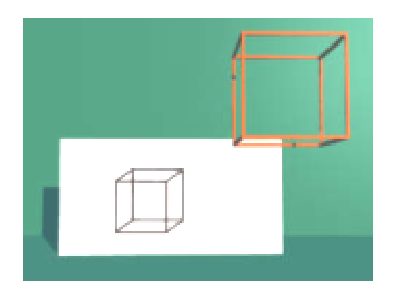
\includegraphics[scale=0.66]{./Graphiques/Perspective1.eps}
	\end{center}
 \end{minipage}

\end{tabular}

      \end{encadrer}
%\end{minipage}&
%\begin{minipage}[r]{0.275\linewidth}

	
%\end{minipage}
%\end{tabular}

%\medskip



%      \sautpage

\begin{rmqs}~
\begin{itemize}
\item Il arrivera parfois que le cube soit représenté sans faces parallèles à l'écran.
\item Si les rayons sont perpendiculaires à l'écran, on parle de perspective orthogonale. Dans toute la suite, on exclura ce cas.
\item On parle d'\textbf{une} représentation en perspective cavalière, car la forme de l'ombre dépend de la direction des rayons du soleil.
      \begin{center}
	  \begin{tabular}{cc}
	  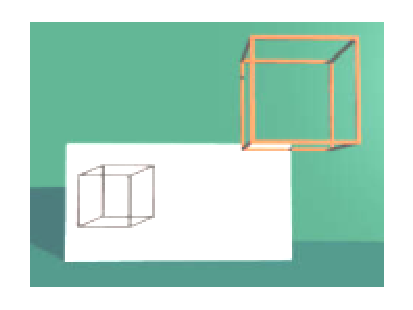
\includegraphics[scale=0.66]{./Graphiques/Perspective2.eps}&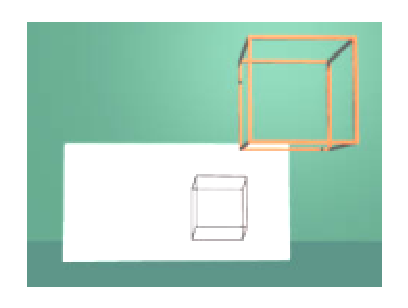
\includegraphics[scale=0.66]{./Graphiques/Perspective3.eps}
	  \end{tabular}
      \end{center}

\end{itemize}
\end{rmqs}

\begin{encadrer}
\begin{tabular}{cc}
\begin{minipage}[l]{0.69\linewidth}
 \emph{On appelle \emph{fuyante} une droite perpendiculaire à l'écran.\\
      Les ombres de toutes les fuyantes sont parallèles et leur direction commune dépend de celle des rayons du soleil.}
\end{minipage}&
\begin{minipage}[r]{0.30\linewidth}
 \begin{center}
	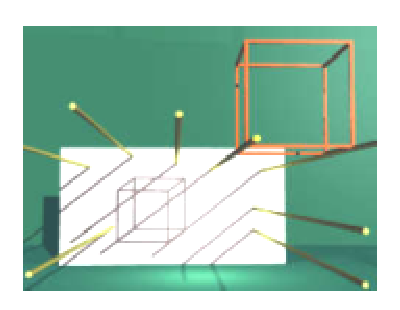
\includegraphics[scale=0.66]{./Graphiques/Perspective4.eps}
	\end{center}
\end{minipage}
\end{tabular}
\end{encadrer}



\subsection{Construction et propriétés}

\subsubsection{Construction}

\begin{tabular}{cc}
\begin{minipage}[l]{0.75\linewidth}
\begin{itemize}
\item L'angle $\alpha$ des fuyantes (droites perpendiculaires au plan de projection) vaut habituellement 30°, 45° ou 60°.
\item Toutes les dimensions qui sont dans des plans parallèles au plan de projection sont représentées en vraie grandeur.
\item Les dimensions qui sont portées par les fuyantes sont multipliées par un coefficient de réduction, en général compris entre 0,5 et 0,8.
\end{itemize}
\end{minipage}&
\begin{minipage}[r]{0.25\linewidth}
\begin{center}
\psset{xunit=0.5cm , yunit=0.5cm}
\begin{pspicture*}(-0.7,-0.7)(6.7,5.7)
\def\xmin{-0.5} \def\xmax{6.5} \def\ymin{-0.5} \def\ymax{5.5}

\psset{linecolor=black, linewidth=.5pt, arrowsize=2pt 4}
\psline(0.0000,0.0000)(4.0000,0.0000)
\psline(4.0000,0.0000)(4.0000,4.0000)
\psline(4.0000,4.0000)(0.0000,4.0000)
\psline(0.0000,4.0000)(0.0000,0.0000)
\psline[linestyle=dashed](2.0000,1.0000)(6.0000,1.0000)
\psline(6.0000,1.0000)(6.0000,5.0000)
\psline(6.0000,5.0000)(2.0000,5.0000)
\psline[linestyle=dashed](2.0000,5.0000)(2.0000,1.0000)
\psline[linestyle=dashed](0.0000,0.0000)(2.0000,1.0000)
\psline(4.0000,0.0000)(6.0000,1.0000)
\psline(4.0000,4.0000)(6.0000,5.0000)
\psline(0.0000,4.0000)(2.0000,5.0000)
\psarc(0.0000,4.0000){0.4500}{0.0000}{26.5651}
\psarc(0.0000,4.0000){0.5500}{0.0000}{26.5651}
\rput(1.4,4.3){$\alpha$}

\end{pspicture*}
\end{center}
\end{minipage}
\end{tabular}



\subsubsection{Propriétés}

\begin{encadrer}
\begin{itemize}
\item \emph{Des droites parallèles sont représentées sur le dessin par des droites parallèles.}
\item \emph{Des droites sécantes sont représentées sur le dessin par des droites sécantes.}
\item \emph{Les rapports de longueur sur une droite sont conservés sur le dessin.\\ Ainsi, par exemple, le milieu d'un segment est représenté sur le dessin par le milieu du segment obtenu.}
\end{itemize}
\end{encadrer}




\begin{rmqs} Attention, les r\'eciproques ne sont pas vraies. Ainsi :
\begin{itemize}
 \item Deux droites qui semblent parallèles sur le dessin ne le sont pas toujours dans la réalité.
 \item Deux droites qui semblent sécantes sur le dessin ne le sont pas toujours dans la réalité.
 \item Un point qui semble \^etre au milieu d'un segment dans la repr\'esentation en perspective cavali\`ere n'est pas toujours le milieu du segment dans la r\'ealit\'e : il peut ne pas \^etre sur le segment dans la r\'ealit\'e.
\end{itemize}

 
\end{rmqs}


%\sautpage

\section{Solides usuels et volumes}


\subsection{Famille des prismes droits}

\begin{center}
\begin{tabular}{p{5cm} p{5cm} p{5cm}}
\textbf{Prisme droit} & \textbf{Pavé} & \textbf{Cylindre} \\
Toutes les faces sont des rectangles sauf (éventuellement) les deux bases. & Prisme droit dont les bases sont des rectangles. & Peut être considéré comme un prisme droit dont les bases sont des disques. \\
\end{tabular}
\end{center}

\begin{multicols}{3}
\begin{center}
\psset{xunit=0.75cm , yunit=0.375cm}
\begin{pspicture*}(-0.7,-0.7)(5.7,5.7)
\def\xmin{-0.5} \def\xmax{5.5} \def\ymin{-0.5} \def\ymax{5.5}

\psset{linecolor=black, linewidth=.5pt, arrowsize=2pt 4}
\psline(0.0000,1.0000)(3.0000,0.0000)
\psline(3.0000,0.0000)(5.0000,1.0000)
\psline[linestyle=dashed](5.0000,1.0000)(4.0000,2.0000)
\psline[linestyle=dashed](4.0000,2.0000)(2.0000,2.0000)
\psline[linestyle=dashed](2.0000,2.0000)(0.0000,1.0000)
\psline(0.0000,4.0000)(3.0000,3.0000)
\psline(0.0000,1.0000)(0.0000,4.0000)
\psline(3.0000,0.0000)(3.0000,3.0000)
\psline(3.0000,3.0000)(5.0000,4.0000)
\psline(5.0000,1.0000)(5.0000,4.0000)
\psline(5.0000,4.0000)(4.0000,5.0000)
\psline[linestyle=dashed](4.0000,2.0000)(4.0000,5.0000)
\psline(4.0000,5.0000)(2.0000,5.0000)
\psline(2.0000,5.0000)(0.0000,4.0000)
\psline[linestyle=dashed](2.0000,5.0000)(2.0000,2.0000)
\rput(2.5,1.3){\emph{base}}
\psline{<->}(-0.2,1)(-0.2,4)
\rput(-0.4,2.5){$h$}

\end{pspicture*}
\end{center}
\sautcol

\begin{center}
\psset{xunit=0.75cm , yunit=0.375cm}
\begin{pspicture*}(-0.7,-0.7)(5.7,5.7)
\def\xmin{-0.5} \def\xmax{5.5} \def\ymin{-0.5} \def\ymax{5.5}

\psset{linecolor=black, linewidth=.5pt, arrowsize=2pt 4}
\psline(0.0000,0.0000)(3.0000,0.0000)
\psline(3.0000,0.0000)(3.0000,3.0000)
\psline(3.0000,3.0000)(0.0000,3.0000)
\psline(0.0000,3.0000)(0.0000,0.0000)
\psline[linestyle=dashed](2.0000,1.0000)(5.0000,1.0000)
\psline(5.0000,1.0000)(5.0000,4.0000)
\psline(5.0000,4.0000)(2.0000,4.0000)
\psline[linestyle=dashed](2.0000,4.0000)(2.0000,1.0000)
\psline[linestyle=dashed](0.0000,0.0000)(2.0000,1.0000)
\psline(3.0000,0.0000)(5.0000,1.0000)
\psline(3.0000,3.0000)(5.0000,4.0000)
\psline(0.0000,3.0000)(2.0000,4.0000)
\rput(2.3,0.5){\emph{base}}
\psline{<->}(-0.2,0)(-0.2,3)
\rput(-0.4,1.5){$h$}

\end{pspicture*}
\end{center}
\sautcol

\begin{center}
\psset{xunit=0.75cm , yunit=0.1875cm}
\begin{pspicture*}(-0.6,-1.2)(5.6,11.1)
\def\xmin{-0.5} \def\xmax{5.5} \def\ymin{-1.1} \def\ymax{11}

\def\F{1 4 x 2 sub 2 exp sub 0.5 exp add}
\psplot[linecolor=black,linestyle=dashed]{0}{4}{\F}
\def\G{1 4 x 2 sub 2 exp sub 0.5 exp sub}
\psplot[linecolor=black,linestyle=solid]{0}{4}{\G}
\def\H{8 4 x 2 sub 2 exp sub 0.5 exp add}
\psplot[linecolor=black,linestyle=solid]{0}{4}{\H}
\def\I{8 4 x 2 sub 2 exp sub 0.5 exp sub}
\psplot[linecolor=black,linestyle=solid]{0}{4}{\I}
\psline(0,1)(0,8)
\psline(4,1)(4,8)
\rput(2,1){\emph{base}}
\psline{<->}(4.5,1)(4.5,8)
\rput(5,4.5){$h$}

\end{pspicture*}
\end{center}
\end{multicols}

\begin{prop}
 Le volume de ces solides est donné par la formule suivante : \[\text{Volume}=\text{Aire de la base}\times\text{hauteur}\]
\end{prop}

\subsection{Famille des pyramides}

\begin{center}
\begin{tabular}{p{5cm} p{5cm} p{5cm}}
\textbf{Pyramide} & \textbf{Tétraèdre} & \textbf{Cône de révolution} \\
Constituée d'une base de forme quelconque et d'un sommet. Des arêtes joignent ce sommet à chacun des sommets de la base. & Pyramide dont la base est un triangle. & Peut être considéré comme une pyramide dont la base est un disque. \\
\end{tabular}
\end{center}

\begin{multicols}{3}
\begin{center}
\psset{xunit=0.75cm , yunit=0.375cm}
\begin{pspicture*}(-0.7,-0.7)(5.7,5.7)
\def\xmin{-0.5} \def\xmax{5.5} \def\ymin{-0.5} \def\ymax{5.5}

\psset{linecolor=black, linewidth=.5pt, arrowsize=2pt 4}
\psline(0.0000,1.0000)(2.0000,0.0000)
\psline(2.0000,0.0000)(4.0000,1.0000)
\psline[linestyle=dashed](4.0000,1.0000)(3.0000,2.0000)
\psline[linestyle=dashed](3.0000,2.0000)(1.0000,2.0000)
\psline[linestyle=dashed](1.0000,2.0000)(0.0000,1.0000)
\psline(0.0000,1.0000)(2.0000,5.0000)
\psline(2.0000,0.0000)(2.0000,5.0000)
\psline(4.0000,1.0000)(2.0000,5.0000)
\psline[linestyle=dashed](3.0000,2.0000)(2.0000,5.0000)
\psline[linestyle=dashed](1.0000,2.0000)(2.0000,5.0000)
\rput(2,1){\emph{base}}
\psline{<->}(4.3,1)(4.3,5)
\psline[linestyle=dotted](2,5)(4.3,5)
\rput(4.5,3){$h$}

\end{pspicture*}
\end{center}
\sautcol

\begin{center}
\psset{xunit=0.75cm , yunit=0.375cm}
\begin{pspicture*}(-0.7,-0.7)(5.7,5.7)
\def\xmin{-0.5} \def\xmax{5.5} \def\ymin{-0.5} \def\ymax{5.5}

\psset{linecolor=black, linewidth=.5pt, arrowsize=2pt 4}
\psline(0.0000,1.0000)(3.0000,0.0000)
\psline[linestyle=dashed](0.0000,1.0000)(4.0000,2.0000)
\psline(3.0000,0.0000)(4.0000,2.0000)
\psline(0.0000,1.0000)(2.0000,5.0000)
\psline(3.0000,0.0000)(2.0000,5.0000)
\psline(4.0000,2.0000)(2.0000,5.0000)
\rput(2.5,0.9){\emph{base}}
\psline{<->}(4.5,1)(4.5,5)
\rput(4.7,3){$h$}
\psline[linestyle=dotted](2,5)(4.5,5)

\end{pspicture*}
\end{center}
\sautcol

\begin{center}
\psset{xunit=0.75cm , yunit=0.1875cm}
\begin{pspicture*}(-0.6,-1.2)(5.6,11.1)
\def\xmin{-0.5} \def\xmax{5.5} \def\ymin{-1.1} \def\ymax{11}

\def\F{1 4 x 2 sub 2 exp sub 0.5 exp add}
\psplot[linecolor=black,linestyle=dashed]{0}{4}{\F}
\def\G{1 4 x 2 sub 2 exp sub 0.5 exp sub}
\psplot[linecolor=black,linestyle=solid]{0}{4}{\G}
\psline(0,1)(2,8)(4,1)
\rput(2,1){\emph{base}}
\psline{<->}(4.5,1)(4.5,8)
\rput(5,4.5){$h$}
\psline[linestyle=dotted](2,8)(4.5,8)
\end{pspicture*}
\end{center}
\end{multicols}

\begin{prop}
 Le volume de ces solides est donné par la formule suivante : \[\text{Volume}=\frac{1}{3}\text{Aire de la base}\times\text{hauteur}\]

\end{prop}

On peut ainsi mettre trois fois le volume d'un cône de révolution dans un cylindre de révolution ayant même base et même hauteur, ou trois fois le volume d'un tétraèdre dans un prisme droit ayant même base et même hauteur.

\subsection{Sphère}

\begin{tabular}{cc}
\begin{minipage}[l]{0.7\linewidth}
\begin{prop}
 Le volume d'une sph\`ere de rayon $r$ est donn\'e par la formule : \[\text{Volume}=\frac{4}{3}\pi r^3\]
 L'aire de la surface d'une sph\`ere de rayon $r$ est donn\'ee par la formule : \[\text{Aire}=4\pi r^2\]
\end{prop}
\end{minipage}&
\begin{minipage}[r]{0.3\linewidth}
\begin{center}
\psset{xunit=0.66cm , yunit=0.66cm}
\begin{pspicture*}(-3.6,-3.6)(3.6,3.6)
\def\xmin{-3.5} \def\xmax{3.5} \def\ymin{-3.5} \def\ymax{3.5}

\def\F{9 x 2 exp sub 0.5 exp}
\psplot[linecolor=black,linestyle=solid]{-3}{3}{\F}
\def\G{0 9 x 2 exp sub 0.5 exp sub}
\psplot[linecolor=black,linestyle=solid]{-3}{3}{\G}
\def\H{1 3 div 9 x 2 exp sub 0.5 exp mul}
\psplot[linecolor=black,linestyle=dashed]{-3}{3}{\H}
\def\I{0 1 3 div 9 x 2 exp sub 0.5 exp mul sub}
\psplot[linecolor=black,linestyle=solid]{-3}{3}{\I}
\psline[linestyle=dashed]{o-}(0,0)(3,0)
\rput(-0.3,-0.3){$O$}
\rput(1.5,0.3){$r$}

\end{pspicture*}
\end{center}
\end{minipage}
\end{tabular}



\section{Incidence et parall\'elisme dans l'espace}

\subsection{Règles d'incidence}

\begin{regle}
Par deux points distincts de l'espace $A$ et $B$, il passe une unique droite, notée $(AB)$.
\end{regle}

\begin{regle}
Par trois points non alignés de l'espace $A$, $B$ et $C$, il passe un unique plan, noté $(ABC)$.
\end{regle}

\begin{regle}
Si deux points distincts $A$ et $B$ de l'espace appartiennent à un plan $\mathcal{P}$, alors la droite $(AB)$ est contenue dans le plan $\mathcal{P}$, c'est-à-dire que tout point $M$ appartenant à la droite $(AB)$ appartient aussi au plan $\mathcal{P}$.
\end{regle}

\begin{regle}
Dans chaque plan de l'espace, on peut appliquer tous les théorèmes de géométrie plane (\textsc{Pythagore}, \textsc{Thalès}, etc.).
\end{regle}

\subsection{Postions relatives}
\subsubsection{Positions relatives de deux droites}

\begin{regle}
Deux droites de l'espace sont soit coplanaires, soit non coplanaires.
\end{regle}
\psset{unit=0.75}
\begin{center}
\begin{tabular}{ccc|c}
\multicolumn{3}{c|}{\textbf{Coplanaires (dans un même plan)}}&\textbf{Non coplanaires} \\\hline
$d$ et $d'$ sécantes & \multicolumn{2}{c|}{$d$ et $d'$ parallèles}& \\
\begin{pspicture*}(-0.6,-2.7)(4.2,1.2)
\psline[linecolor=gray](0,0)(0,-2)(2,-2)(2,0)(0,0)(1,0.5)(3,0.5)(3,-1.5)(2,-2)
\psline[linecolor=gray](2,0)(3,0.5)
\psline(0,0.5)(3.5,0.5) \uput[u](0,0.4){$d$}
\psplot[algebraic=true,plotpoints=200]{-0.5}{4}{x/6} \uput[u](-0.1,-0.2){$d'$}
\psdot[dotstyle=x](3,0.5) \uput[u](3,0.5){$A$}
\end{pspicture*}
&
\begin{pspicture*}(-0.6,-2.7)(4.2,1.2)
\psline[linecolor=gray](0,0)(0,-2)(2,-2)(2,0)(0,0)(1,0.5)(3,0.5)(3,-1.5)(2,-2)
\psline[linecolor=gray](2,0)(3,0.5)
\psline(0,0.5)(3.7,0.5) \uput[u](0,0.4){$d$}
\psline(-0.5,0)(3.2,0) \uput[u](-0.3,-0.1){$d'$}
\end{pspicture*}
&
\begin{pspicture*}(-0.6,-2.7)(4.2,1.2)
\psline[linecolor=gray](0,0)(0,-2)(2,-2)(2,0)(0,0)(1,0.5)(3,0.5)(3,-1.5)(2,-2)
\psline[linecolor=gray](2,0)(3,0.5)
\psline(-0.5,0.005)(3.2,0.005) \uput[u](-0.3,-0.1){$d$}
\psline(-0.5,-0.005)(3.2,-0.005) \uput[d](3,0.1){$d'$}
\end{pspicture*}
&
\begin{pspicture*}(-0.6,-2.7)(4.2,1.2)
\psline[linecolor=gray](0,0)(0,-2)(2,-2)(2,0)(0,0)(1,0.5)(3,0.5)(3,-1.5)(2,-2)
\psline[linecolor=gray](2,0)(3,0.5)
\psline(-0.5,0)(3.2,0) \uput[u](-0.3,-0.1){$d$}
\psplot[algebraic=true,plotpoints=200]{-0.5}{4}{0.5*x-3} \uput[dl](2.1,-2){$d'$}
\end{pspicture*}\\

\multicolumn{1}{m{3cm}}{$d$ et $d'$ ont un point d'intersubsection $A$.}
& \multicolumn{1}{m{3cm}}{$d$ et $d'$ sont strictement parallèles.} & \multicolumn{1}{m{3cm}|}{$d$ et $d'$ sont confondues} & \multicolumn{1}{m{3cm}}{Aucun plan ne contient à la fois $d$ et $d'$.} \\
$d\cap d' = \{ A \}$ & $d\cap d' = \vide$ & $d\cap d' = d=d'$ & $d\cap d' = \vide$\\
\end{tabular}
\end{center}

%\sautpage

\begin{rmqs}~
\begin{itemize}
\item Contrairement au plan, deux droites de l'espace n'ayant pas de point en commun ne sont pas forcément parallèles.
\item Des droites strictement parallèles sont des droites \textbf{coplanaires et qui n'ont aucun point en commun}.
	\item On peut définir un plan de plusieurs manières :
			\begin{itemize}
				\item par la donnée de trois points ;
				\item par la donné de deux droites sécantes ;
				\item par la donnée de deux droites strictement parallèles ;
				\item par la donnée d'une droite et d'un point n'appartenant par à cette droite.
			\end{itemize}
\end{itemize}
\end{rmqs}

\sautpage

\subsubsection{Positions relatives d'une droite et d'un plan}

\begin{regle}
Une droite et un plan de l'espace sont soit sécants, soit parallèles.
\end{regle}

\psset{unit=1}
\begin{center}
\begin{tabular}{c|cc}
\textbf{Sécants}&\multicolumn{2}{c}{\textbf{Parallèles}} \\\hline
\begin{pspicture*}(-0.6,-0.7)(5.5,2.8)
\pspolygon[fillstyle=solid,fillcolor=lightgray](0,0)(3,0)(5,1)(2,1)
\pspolygon*[linecolor=white](2,0.5)(3,0.5)(3.5,0.75)(3.5,1.75)(2.5,1.75)(2,1.5)
\psline[linecolor=gray,linestyle=dotted](2,0.5)(2.5,0.75)(2.5,1.75)
\psline[linecolor=gray,linestyle=dotted](2.5,0.75)(3.5,0.75)
\psline[linecolor=gray](2,1.5)(2,0.5)(3,0.5)(3,1.5)(2,1.5)(2.5,1.75)(3.5,1.75)(3.5,0.75)(3,0.5)
\psline[linecolor=gray](3,1.5)(3.5,1.75)
\psplot[linestyle=dotted,algebraic=true,plotpoints=200]{2.5}{3.866}{-x+4.25}
\psplot[algebraic=true,plotpoints=200]{1.5}{2.5}{-x+4.25}
\psplot[algebraic=true,plotpoints=200]{3.866}{4.75}{-x+4.25}
\psdot[dotstyle=x](3.5,0.75)
\uput[r](3.5,0.75){$B$}
\uput[u](4.6,-0.4){$d$}
\uput[u](4.6,1){$\mathcal{P}$}
\end{pspicture*}
&
\begin{pspicture*}(-0.6,-0.7)(5.5,2.8)
\pspolygon[fillstyle=solid,fillcolor=lightgray](0,0)(3,0)(5,1)(2,1)
\pspolygon*[linecolor=white](2,0.5)(3,0.5)(3.5,0.75)(3.5,1.75)(2.5,1.75)(2,1.5)
\psline[linecolor=gray,linestyle=dotted](2,0.5)(2.5,0.75)(2.5,1.75)
\psline[linecolor=gray,linestyle=dotted](2.5,0.75)(3.5,0.75)
\psline[linecolor=gray](2,1.5)(2,0.5)(3,0.5)(3,1.5)(2,1.5)(2.5,1.75)(3.5,1.75)(3.5,0.75)(3,0.5)
\psline[linecolor=gray](3,1.5)(3.5,1.75)
\psline(0,1.75)(4.5,1.75)
\uput[l](0,1.75){$d$}
\uput[u](4.6,1){$\mathcal{P}$}
\end{pspicture*}
&
\begin{pspicture*}(-0.6,-0.7)(5.5,2.8)
\pspolygon[fillstyle=solid,fillcolor=lightgray](0,0)(3,0)(5,1)(2,1)
\pspolygon*[linecolor=white](2,0.5)(3,0.5)(3.5,0.75)(3.5,1.75)(2.5,1.75)(2,1.5)
\psline[linecolor=gray,linestyle=dotted](2,0.5)(2.5,0.75)(2.5,1.75)
\psline[linecolor=gray,linestyle=dotted](2.5,0.75)(3.5,0.75)
\psline[linecolor=gray](2,1.5)(2,0.5)(3,0.5)(3,1.5)(2,1.5)(2.5,1.75)(3.5,1.75)(3.5,0.75)(3,0.5)
\psline[linecolor=gray](3,1.5)(3.5,1.75)
\psline(0,0.5)(4.5,0.5)
\uput[l](0,0.5){$d$}
\uput[u](4.6,1){$\mathcal{P}$}
\end{pspicture*}
\\
\multicolumn{1}{m{4cm}|}{$d$ et $\mathcal{P}$ ont un point d'intersubsection $B$.}
& \multicolumn{1}{m{4cm}}{$d$ et $\mathcal{P}$ sont strictement parallèles.} & \multicolumn{1}{m{4cm}}{$d$ est contenue dans $\mathcal{P}$} \\
$d\cap \mathcal{P} = \{ B \}$ & $d\cap \mathcal{P} = \vide$ & $d\cap \mathcal{P} = d$\\
\end{tabular}
\end{center}

\begin{rmq} Une droite $d$ et un plan $\mathcal{P}$ sont parallèles s'ils ne sont pas sécants. On note alors $d\parallel \mathcal{P}$ ou $\mathcal{P}\parallel d$.
\end{rmq}

\subsubsection{Positions relatives de deux plans}

\begin{regle}
Deux plans de l'espace sont soit sécants, soit parallèles.
\end{regle}

\psset{unit=1}
\begin{center}
\begin{tabular}{c|cc}
\textbf{Sécants}&\multicolumn{2}{c}{\textbf{Parallèles}} \\\hline
\begin{pspicture*}(-0.6,-0.7)(6,2.8)
\pspolygon[fillstyle=solid,fillcolor=gray](0,0)(3,0)(5,1)(2,1)
\pspolygon[fillstyle=solid,fillcolor=lightgray](5,1)(2,1)(0,4)(3,4)
\pspolygon*[linecolor=white](2.5,1.75)(2.5,0.75)(3.5,0.75)(4,1)(3.5,1.75)
\psline(3.5,0.75)(4,1)(3.5,1.75)(3.5,0.75)(2.5,0.75)(2.5,1.75)(3.5,1.75)
\psline[linestyle=dotted](2.5,0.75)(3,1)(3,2)(2.5,1.75)(3,1)(4,1)(4,2)(3.5,1.75)
\psline[linestyle=dotted](3,2)(4,2)
\psline[linestyle=dotted](2.5,1)(3,1)
\psline(1,1)(2,1)\uput[l](1,1){$d$}
\psline(5,1)(5.5,1)
\uput[u](0,0){$\mathcal{P}$}
\uput[dl](1,2.5){$\mathcal{P}'$}
\end{pspicture*}
&
\begin{pspicture*}(-0.6,-0.7)(6,2.8)
\pspolygon[fillstyle=solid,fillcolor=gray](0,0)(3,0)(5,1)(2,1)
\pspolygon[fillstyle=solid,fillcolor=lightgray](0,1.5)(3,1.5)(5,2.5)(2,2.5)
\pspolygon*[linecolor=white](1.5,1.75)(2.5,1.75)(3,2)(2,2)
\pspolygon*[linecolor=white](1.5,0.25)(2.5,0.25)(3,0.5)(3,1.25)(1.5,1.25)
\psline[linestyle=dotted](2,2)(2,0.5)(1.5,0.25)
\psline[linestyle=dotted](2,0.5)(3,0.5)
\psline[linestyle=dotted](1.5,1.75)(1.5,1.5)
\psline[linestyle=dotted](2.5,1.75)(2.5,1.5)
\psline[linestyle=dotted](3,2)(3,1.5)
\psline(1.5,1.5)(1.5,0.25)(2.5,0.25)(2.5,1.5)
\psline(2.5,0.25)(3,0.5)(3,1.5)
\psline(1.5,1.75)(2.5,1.75)(3,2)(2,2)(1.5,1.75)
\uput[u](0,0){$\mathcal{P}$}
\uput[u](0,1.5){$\mathcal{P}'$}
\end{pspicture*}
&
\begin{pspicture*}(-1.4,-0.7)(6.5,2.8)
\pspolygon[fillstyle=solid,fillcolor=gray](-1,-0.25)(3.25,-.25)(6.25,1.25)(2,1.25)
\pspolygon[fillstyle=solid,fillcolor=lightgray](0,0)(3,0)(5,1)(2,1)
\pspolygon*[linecolor=white](2,0.5)(3,0.5)(3.5,0.75)(3.5,1.75)(2.5,1.75)(2,1.5)
\psline[linecolor=gray,linestyle=dotted](2,0.5)(2.5,0.75)(2.5,1.75)
\psline[linecolor=gray,linestyle=dotted](2.5,0.75)(3.5,0.75)
\psline[linecolor=gray](2,1.5)(2,0.5)(3,0.5)(3,1.5)(2,1.5)(2.5,1.75)(3.5,1.75)(3.5,0.75)(3,0.5)
\psline[linecolor=gray](3,1.5)(3.5,1.75)
\uput[u](6,1.25){$\mathcal{P}$}
\rput(4,0.75){$\mathcal{P}'$}
\end{pspicture*}\\
\multicolumn{1}{m{4cm}|}{$\mathcal{P}$ et $\mathcal{P}'$ ont une droite d'intersubsection $d$.}
& \multicolumn{1}{m{4cm}}{$\mathcal{P}$ et $\mathcal{P}'$ sont strictement parallèles.} & \multicolumn{1}{m{4cm}}{$\mathcal{P}$ et $\mathcal{P}'$ sont confondus} \\
$\mathcal{P}\cap \mathcal{P}' = d$ & $\mathcal{P}\cap \mathcal{P}' = \vide$ & $\mathcal{P}\cap \mathcal{P}' = \mathcal{P}= \mathcal{P}'$\\
\end{tabular}
\end{center}
\begin{rmq}Deux plans $\mathcal{P}$ et $\mathcal{P}'$ sont parallèles lorsqu'ils ne sont pas sécants. On note $\mathcal{P}\parallel \mathcal{P}'$.
\end{rmq}

\begin{rmqs}~
\begin{itemize}
	\item Pour démontrer que trois points sont alignés, il suffit de montrer que les trois points appartiennent à deux plans sécants : comme l'intersubsection de deux plans sécants est une droite, cela implique que les points sont tous les trois sur cette droite.
	\item Pour trouver la droite d'intersubsection de deux plans, il suffit de trouver deux points distincts qui appartiennent aux deux plans : la droite d'intersubsection est alors celle qui passe par ces deux points. Ces points sont en général des points d'intersubsection de droites sécantes, l'une contenue dans l'un des plans, l'autre dans l'autre plan.
\end{itemize}
\end{rmqs}

%\sautpage

\subsection{Parallélisme dans l'espace}

\subsubsection{Parallélisme entre droites}

\begin{prop} Deux droites parallèles à une même droite sont parallèles entre elles.
\[ \text{Si } d \parallel  d' \text{ et } d'\parallel d'' \text{ alors } d\parallel d''\]
\end{prop}

\begin{prop}
Si deux droites sont parallèles, alors tout plan qui coupe l'une, coupe l'autre.
\end{prop}

\subsubsection{Parallélisme entre plans}

\begin{prop} Deux plans parallèles à un même plan sont parallèles entre eux.
\[ \text{Si } \mathcal{P} \parallel  \mathcal{P}' \text{ et } \mathcal{P}'\parallel \mathcal{P}'' \text{ alors } \mathcal{P}\parallel \mathcal{P}''\]
\end{prop}

\begin{prop}
Si deux droites sécantes $d$ et $d'$ d'un plan $\mathcal{P}$ sont parallèles à deux droites sécantes $\Delta$ et $\Delta '$ d'un plan $\mathcal{Q}$, alors $\mathcal{P}$ et $\mathcal{Q}$ sont parallèles.
\end{prop}

\begin{center}
\psset{xunit=2cm,yunit=1cm}
\begin{pspicture*}(-0.6,-0.7)(6,2.8)
\pspolygon[fillstyle=solid](0,0)(3,0)(5,1)(2,1)
\pspolygon[fillstyle=solid](0,1.5)(3,1.5)(5,2.5)(2,2.5)
\psline(0.5,0.1)(4.2,0.9) \uput[r](4.2,0.9){$d$}
\psline(0.5,1.6)(4.2,2.4) \uput[r](4.2,2.4){$\Delta$}
\psline(1.5,0.6)(2.6,0.1) \uput[ur](2.6,0.1){$d'$}
\psline(1.9,2.4)(3,1.9) \uput[r](2.9,1.9){$\Delta '$}
\uput[u](0,0){$\mathcal{P}$}
\uput[u](0,1.5){$\mathcal{Q}$}
\end{pspicture*}
\end{center}

\begin{prop}
Si deux plans $\mathcal{P}$ et $\mathcal{P}'$ sont parallèles, alors tout plan sécant à $\mathcal{P}$ est aussi sécant à $\mathcal{P}'$ et leurs droites d'intersubsection $d$ et $d'$ sont parallèles.
\end{prop}

\begin{center}
\psset{xunit=1.5cm,yunit=0.5cm}
\begin{pspicture*}(-1,-3.5)(6.5,8.5)
\pspolygon[fillstyle=solid,fillcolor=lightgray,linecolor=black](0,-3)(2,-1)(5,8)(3,6)
\pspolygon*[linecolor=white](1,0)(2.3333,0)(3,2)
\pspolygon*[linecolor=white](2,3)(3.3333,3)(4,5)
\psline(1.6667,2)(1,2)(0,0)(5,0)(6,2)(3,2)
\psline(2.6667,5)(1,5)(0,3)(5,3)(6,5)(4,5)
\uput[l](0,0){$\mathcal{P}$}
\uput[l](0,3){$\mathcal{Q}$}
\psline(0.5,-0.5)(3.5,2.5)\uput[l](0.5,-0.5){$d$}
\psline(1.5,2.5)(4.5,5.5)\uput[l](1.5,2.5){$d'$}
\psline[linestyle=dotted](2.3333,0)(3,2)(1.6667,2)
\psline[linestyle=dotted](3.3333,3)(4,5)(2.6667,5)
\end{pspicture*}
\end{center}


\subsubsection{Parallélisme entre droite et plan}

\begin{prop}
Si deux plans $\mathcal{P}$ et $\mathcal{P}'$ sont parallèles et si une droite $d$ est parallèle à $\mathcal{P}$, alors $d$ est parallèle à $\mathcal{P}'$.
\[ \text{Si } d\parallel \mathcal{P} \text{ et } \mathcal{P}\parallel \mathcal{P}' \text{ alors } d\parallel \mathcal{P}'\]
\end{prop}

\begin{center}
\psset{xunit=1.5cm,yunit=1cm}
\begin{pspicture*}(-0.6,-0.7)(6,3.9)
\pspolygon[fillstyle=solid](0,0)(3,0)(5,1)(2,1)
\pspolygon[fillstyle=solid](0,1.5)(3,1.5)(5,2.5)(2,2.5)
\psline(0.5,3)(4.2,3.5) \uput[l](0.5,3){$d$}
\uput[u](0,0){$\mathcal{P}$}
\uput[u](0,1.5){$\mathcal{P}'$}
\end{pspicture*}
\end{center}

\sautpage

\begin{prop}
Si deux droites $d$ et $\Delta$ sont parallèles, et si $d$ est contenue dans un plan $\mathcal{P}$, alors $\Delta$ est parallèle à $\mathcal{P}$.
\end{prop}

\begin{center}
\psset{xunit=1.5cm,yunit=1cm}
\begin{pspicture*}(-0.6,-0.7)(6,3.9)
\pspolygon[fillstyle=solid](0,1.5)(3,1.5)(5,2.5)(2,2.5)
\psline(0.5,1.6)(4.2,2.4) \uput[r](4.2,2.4){$d$}
\psline(0.5,0.1)(4.2,0.9) \uput[r](4.2,0.9){$\Delta$}
\uput[u](0,1.5){$\mathcal{P}$}
\end{pspicture*}
\end{center}

\begin{prop}
Si deux plans $\mathcal{P}$ et $\mathcal{P}'$ sont sécants selon une droite $\Delta$ et si $d$ est une droite parallèle à $\mathcal{P}$ et $\mathcal{P}'$ alors $d$ et $\Delta$ sont parallèles.
\end{prop}

\begin{center}
\psset{xunit=1.5cm,yunit=0.5cm}
\begin{pspicture*}(-0.6,-2.7)(5.6,7.6)
\pspolygon[fillstyle=solid,fillcolor=gray](0,0)(4,2)(4,7)(0,5)
\pspolygon[fillstyle=solid,fillcolor=lightgray](0,0)(3,-2)(3,3)(0,5)
\uput[r](4,7){$\mathcal{P}'$}
\uput[r](3,-2){$\mathcal{P}$}
\psline(0,-1)(0,6)\uput[u](0,6){$\Delta$}
\psline(5,-1)(5,6)\uput[u](5,6){$d$}
\end{pspicture*}
\end{center}

\begin{theo}[Théorème du toit]
Si :
\begin{itemize}
	\item $d$ et $d'$ sont parallèles ;
	\item $\mathcal{P}$ est un plan qui contient $d$ et $\mathcal{P}'$ est un plan qui contient $d'$ ;
	\item $\mathcal{P}$ et $\mathcal{P}'$ sont sécants selon une droite $\Delta$
\end{itemize}
alors $\Delta$ est parallèle à $d$ et à $d'$.
\end{theo}

\begin{center}
\psset{xunit=1cm,yunit=0.5cm}
\begin{pspicture*}(-0.6,-0.6)(14.6,10.6)
\pspolygon[fillstyle=solid,fillcolor=gray](2,3)(10,7)(11,9)(3,5)
\pspolygon[fillstyle=solid,fillcolor=lightgray](4,1)(12,5)(11,9)(3,5)
\uput[ul](2,3){$\mathcal{P}'$}
\uput[ur](12,5){$\mathcal{P}$}
\psline(2,0)(14,6)\uput[ul](2,0){$d$}
\psline(0,2)(3.33333,3.66667)\uput[ul](0,2){$d'$}
\psline(1,4)(13,10)\uput[ul](1,4){$\Delta$}
\psline[linestyle=dotted](3.33333,3.66667)(11.3333333,7.666667)
\psline(11.3333333,7.666667)(12,8)
\psline[linestyle=dotted](10,7)(11,9)
\end{pspicture*}
\end{center}

\sautpage

\section{Exercices}

\subsection{Perspective et calculs}


\begin{exo}



Une pièce métallique (en traits pleins) est découpée dans un cube. 

\begin{center}
		\includegraphics[width=0.4\textwidth]{./Graphiques/piece.eps}\end{center}

Construire, en perspective cavalière : 
\vspace{-1.5em}\begin{multicols}{2}
\begin{itemize}
 \item la pièce restante du cube la face $ABCD$ restant devant ;
 \begin{center}
\includegraphics{./Graphiques/piece2.eps} \end{center}

 \item la pièce restante du cube la face $ABCD$ étant à droite. 
 \begin{center}
\includegraphics{./Graphiques/piece3.eps} \end{center}
\end{itemize}
\end{multicols}\vspace{-1.5em}
\end{exo}

%\subsection{Calculs}

\begin{exo}


On considère un tétraèdre $ABCD$, dont les faces $ABC$, $ABD$ et $ACD$ sont des triangles rectangles en $A$.\\
On donne $AB = AD = 5$ cm et $AC = 12$ cm.
\begin{enumerate}
	\item Dessiner ce tétraèdre en perspective cavalière, la face $ABC$ étant frontale.
	\item Quelle est la nature de $CDB$ ? le représenter en vraie grandeur.
	\item Quel est le volume de $ABCD$ ?
\end{enumerate}
\end{exo}

\begin{exo}$ABCDEFGH$ est un cube d'arête $a$.
\begin{enumerate}
	\item Quelle est la nature du triangle $AFC$ ? Justifier. \\
	Le représenter en vraie grandeur à la règle et au compas en prenant $a = 6$ cm.
	\item Calculer la longueur d'une diagonale principale du cube.
\end{enumerate}
\end{exo}

\sautpage

\begin{exo}
On considère un cube $ABCDEFGH$ de côté $a$.
On nomme $P$ le centre de la face $EFGH$ et $Q$ le centre de la face $BCGF$.
$M$ désigne le milieu de $[PQ]$.
On admettra que $(EG)$ est perpendiculaire à $(EA)$ et que $(BG)$ est perpendiculaire à $(AB)$.
\begin{enumerate}
	\item Montrer que $PQ=\frac{a\sqrt{2}}{2}$ puis que $AP=AQ=\frac{a\sqrt{6}}{2}$.
	\item Calculer une valeur approchée au degré près de l'angle $\widehat{PAQ}$.
	\item Donner, en fonction de $a$, la valeur exacte de l'aire du triangle $APQ$.
\end{enumerate}
\end{exo}

\begin{exo}
\begin{multicols}{2}
$ABCDEFGH$ est un parallélépipède rectangle (un pavé) tel que $AB = 10$, $AE = 6$ et $BC = 8$.
\begin{enumerate}
\item Calculer les longueurs des segments $[HA]$, $[HF]$, $[HC]$ et $[HB]$.
\item Calculer le volume des pyramides $HABCD$ et $HBCGF$.
\item Réaliser un patron de ces deux pyramides.
\end{enumerate}
\sautcol
\begin{center}
\psset{xunit=1cm , yunit=0.66cm}
\begin{pspicture*}(-0.7,-0.7)(5.7,5.2)
\def\xmin{-0.5} \def\xmax{5.5} \def\ymin{-0.5} \def\ymax{5}

\psset{linecolor=black, linewidth=.5pt, arrowsize=2pt 4}
\psline(0.0000,0.0000)(3.0000,0.0000)
\psline(3.0000,0.0000)(3.0000,3.0000)
\psline(3.0000,3.0000)(0.0000,3.0000)
\psline(0.0000,3.0000)(0.0000,0.0000)
\psline[linestyle=dashed](2.0000,1.0000)(5.0000,1.0000)
\psline(5.0000,1.0000)(5.0000,4.0000)
\psline(5.0000,4.0000)(2.0000,4.0000)
\psline[linestyle=dashed](2.0000,4.0000)(2.0000,1.0000)
\psline[linestyle=dashed](0.0000,0.0000)(2.0000,1.0000)
\psline(3.0000,0.0000)(5.0000,1.0000)
\psline(3.0000,3.0000)(5.0000,4.0000)
\psline(0.0000,3.0000)(2.0000,4.0000)
\psline[linestyle=dashed](0.0000,0.0000)(2.0000,4.0000)
\psline[linestyle=dashed](3.0000,0.0000)(2.0000,4.0000)
\psline[linestyle=dashed](5.0000,1.0000)(2.0000,4.0000)
\rput(-0.3,-0.3){$A$}
\rput(3,-0.3){$B$}
\rput(5.3,0.7){$C$}
\rput(1.7,1.3){$D$}
\rput(-0.3,3.3){$E$}
\rput(2.7,2.7){$F$}
\rput(5.3,4.3){$G$}
\rput(1.7,4.3){$H$}

\end{pspicture*}
\end{center}
\end{multicols}

\end{exo}



\begin{exo}$ABCDEFGH$ est un cube. $AB$ = 5 cm. Soit $I$ le pied de la hauteur issue de $A$ dans le triangle $ABH$.
\begin{enumerate}
\item Calculer $AH$, $HB$ et $AI$.
\item Représenter en vraie grandeur le triangle $AIC$.
\item Démontrer que la mesure en degrés de $\widehat{AIC}$ est 120°.
\end{enumerate}
\end{exo}

\begin{exo}$SABC$ est un tétraèdre régulier d'arête $a$.
Calculer en fonction de $a$ :
		\begin{enumerate}
		\item la hauteur $SH$ (on admettra que $H$ est l'intersubsection des hauteurs de $ABC$;
		\item l'aire du triangle $ABC$ et l'aire totale du tétraèdre;
		\item le volume du tétraèdre.
		\end{enumerate}
\end{exo}

%\sautpage

\begin{exo}
\begin{multicols}{2}
La figure ci-contre est un patron d'un solide $ABCD$. Le triangle $ADC$ est rectangle en $A$ et a pour dimensions :
\begin{itemize}
\item $AD = 3,5$ cm ;
\item $AC =4$ cm;
\item $AB=3$ cm.
\end{itemize}
\begin{enumerate}
\item De quel type de solide s'agit-il ?
\item Le dessiner en perspective cavalière, en mettant la face $ABC$ en vraie grandeur.
\end{enumerate}

\sautcol

\begin{center}
\psset{xunit=0.7cm , yunit=0.7cm}
\begin{pspicture*}(-0.3,-0.3)(6.2,6)
\def\xmin{-0.1} \def\xmax{6} \def\ymin{-0.1} \def\ymax{5.8}

\psset{linecolor=black, linewidth=.5pt, arrowsize=2pt 4}
\psline(2.0000,2.0000)(2.0000,0.0000)
\psline(2.0000,2.0000)(5.0000,2.0000)
\psline(2.0000,2.0000)(0.0000,2.0000)
\psline(2.0000,2.0000)(2.0000,5.0000)
\psline(2.0000,0.0000)(5.0000,2.0000)
\psline(2.0000,5.0000)(0.0000,2.0000)
\psline(2.0000,5.0000)(5.0000,2.0000)
\psline(2.0000,5.0000)(5.7000,5.7000)
\psline(5.0000,2.0000)(5.7000,5.7000)
\rput(1.7,1.7){$A$}
\rput(5.3,2){$D$}
\rput(2,5.3){$C$}

\end{pspicture*}
\end{center}
\end{multicols}
\end{exo}

\sautpage

\begin{exo}
\begin{multicols}{2}
Soit $SABCD$ une pyramide régulière dont la base est le carré de côté $2a$ et dont les faces latérales sont des triangles isocèles d'angles au sommet de mesure 30°. On désigne respectivement par $I$, $J$ et $H$ les milieux de $[AB]$, $[CD]$ et le centre du carré $ABCD$.
\begin{enumerate}
\item Déterminer, en fonction de $a$, la hauteur $SH$ de cette pyramide.
\item Réaliser un patron de cette pyramide en prenant $a=5$\,cm.
\end{enumerate}

\sautcol

\begin{center}
\psset{xunit=0.75cm , yunit=0.75cm}
\begin{pspicture*}(-0.7,-0.7)(6.7,5.7)
\def\xmin{-0.5} \def\xmax{6.5} \def\ymin{-0.5} \def\ymax{5.5}

\psset{linecolor=black, linewidth=.5pt, arrowsize=2pt 4}
\psline(0.0000,0.0000)(4.0000,0.0000)
\psline(4.0000,0.0000)(6.0000,1.0000)
\psline[linestyle=dashed](6.0000,1.0000)(2.0000,1.0000)
\psline[linestyle=dashed](2.0000,1.0000)(0.0000,0.0000)
\psline(0.0000,0.0000)(3.0000,5.0000)
\psline(4.0000,0.0000)(3.0000,5.0000)
\psline(6.0000,1.0000)(3.0000,5.0000)
\psline[linestyle=dashed](2.0000,1.0000)(3.0000,5.0000)
\psdots[dotstyle=*, dotscale=1.0000](2.0000,0.0000)
\psdots[dotstyle=*, dotscale=1.0000](4.0000,1.0000)
\psdots[dotstyle=*, dotscale=1.0000](3.0000,0.5000)
\psline[linestyle=dashed](3.0000,0.5000)(3.0000,5.0000)
\uput[l](0,0){$A$}
\uput[d](4,0){$B$}
\uput[r](6,1){$C$}
\uput[ul](2,1){$D$}
\uput[u](3,5){$S$}
\uput[d](2,0){$I$}
\uput[u](4,1){$J$}
\uput[r](3,0.5){$H$}
\end{pspicture*}
\end{center}
\end{multicols}
\end{exo}


\begin{exo}
\begin{multicols}{2}
La grande pyramide de Kheops est à sa base un carré presque parfait de 5,3 hectares correctement orienté par rapport au Nord et dont les côtés Nord et Sud sont parallèles à 2,5 cm près. Sa hauteur, à l'origine, était de 146 mètres.
En utilisant la hauteur et les renseignements fournis par le texte ci-dessus, desiner un patron de cette pyramide à l'échelle 1/2600$^e$.\\
Calculer l'aire d'une des faces de la pyramide. \\Comparer le résultat obtenu avec l'aire d'un carré de côté la hauteur de la pyramide.

\sautcol

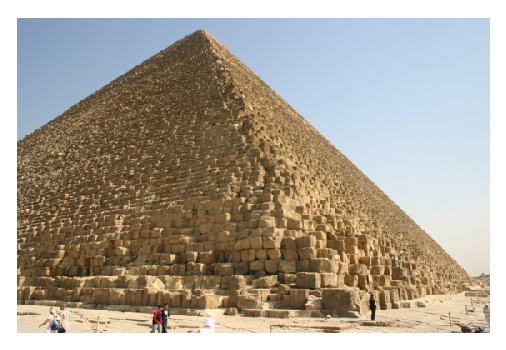
\includegraphics[width=0.45\textwidth]{./Graphiques/kheops.eps}
\end{multicols}
\end{exo}

\begin{exo}
 \begin{multicols}{2}
  $K$ et $L$ sont les milieux des ar\^etes $[EH]$ et $[EF]$ du parall\'el\'epip\`ede rectangle $ABCDEFGH$.
  Les droites $(AK)$ et $(DH)$ se coupent en $M$. Les droites $(AL)$ et $(BF)$ se coupent en $N$.
\begin{enumerate}
 \item D\'emontrer que $K$ est le milieu de $[AM]$.
 \item D\'emontrer que les droites $(KL)$ et $(MN)$ sont parall\`eles.
\end{enumerate}
\sautcol
\begin{center}
\psset{xunit=1cm , yunit=0.75cm}
\def\xmin{-0.5} \def\xmax{5.5} \def\ymin{-2.5} \def\ymax{3}
\begin{pspicture*}(\xmin,\ymin)(\xmax,\ymax)
 \psline(0,2)(0,0)(4,-0.5)(4,1.5)(0,2)(1,2.5)(5,2)(5,0)(4,-0.5)
 \psline(4,1.5)(5,2)
 \psline[linestyle=dashed](0,0)(1,0.5)(1,2.5)
 \psline[linestyle=dashed](1,0.5)(5,0)
 \uput[u](1,2.5){$A$}
 \uput[ur](5,2){$B$}
 \uput[dr](4,1.5){$C$}
 \uput[l](0,2){$D$}
 \uput[ur](1,0.5){$E$}
 \uput[r](5,0){$F$}
 \uput[dl](0,0){$H$}
 \uput[dr](4,-0.5){$G$}

 \psline[linestyle=dotted](1,2.5)(0,-2)(0,0)
 \psline[linestyle=dotted](1,2.5)(5,-2)(5,0)
 \uput[dl](0,-2){$M$}
 \uput[dr](5,-2){$N$}
 \uput[ul](0.5,0.25){$K$}
 \uput[ur](3,0.25){$L$}
\end{pspicture*}
\end{center}
 \end{multicols}

\end{exo}



\begin{exo}
\begin{multicols}{2}
$ABCDEFGH$ est un parallélépipède rectangle (un pavé) tel que $AB = 5$, $AE = 2$ et $BC = 3$.\\
Une fourmi se situe en $E$ et se rend en $C$ en cheminant sur les faces.\\
D\'eterminer le trajet le plus court.\\
\emph{Indication : on pourra s'aider du patron.}
\sautcol
\begin{center}
\psset{xunit=1cm , yunit=0.66cm}
\begin{pspicture*}(-0.7,-0.7)(5.7,5.2)
\def\xmin{-0.5} \def\xmax{5.5} \def\ymin{-0.5} \def\ymax{5}

\psset{linecolor=black, linewidth=.5pt, arrowsize=2pt 4}
\psline(0.0000,0.0000)(3.0000,0.0000)
\psline(3.0000,0.0000)(3.0000,3.0000)
\psline(3.0000,3.0000)(0.0000,3.0000)
\psline(0.0000,3.0000)(0.0000,0.0000)
\psline[linestyle=dashed](2.0000,1.0000)(5.0000,1.0000)
\psline(5.0000,1.0000)(5.0000,4.0000)
\psline(5.0000,4.0000)(2.0000,4.0000)
\psline[linestyle=dashed](2.0000,4.0000)(2.0000,1.0000)
\psline[linestyle=dashed](0.0000,0.0000)(2.0000,1.0000)
\psline(3.0000,0.0000)(5.0000,1.0000)
\psline(3.0000,3.0000)(5.0000,4.0000)
\psline(0.0000,3.0000)(2.0000,4.0000)
%\psline[linestyle=dashed](0.0000,0.0000)(2.0000,4.0000)
%\psline[linestyle=dashed](3.0000,0.0000)(2.0000,4.0000)
%\psline[linestyle=dashed](5.0000,1.0000)(2.0000,4.0000)
\rput(-0.3,-0.3){$A$}
\rput(3,-0.3){$B$}
\rput(5.3,0.7){$C$}
\rput(1.7,1.3){$D$}
\rput(-0.3,3.3){$E$}
\rput(2.7,2.7){$F$}
\rput(5.3,4.3){$G$}
\rput(1.7,4.3){$H$}

\end{pspicture*}
\end{center}
\end{multicols}

\end{exo}


\subsection{Incidence et parall\'elisme}


\begin{tabular}{cc}
 \begin{minipage}[l]{0.625\linewidth}
 \begin{exo}  $SABCD$ est une pyramide \`a base carr\'ee. $I$ est un point du segment $[BC]$, distinct de $B$ et $C$.
\begin{enumerate}
 \item Montrer que les plans $(SAI)$ et $(SCD)$ sont s\'ecants.
 \item Construire leur intersubsection.
\end{enumerate}
\end{exo}
 \end{minipage}
&
\begin{minipage}[r]{0.35\linewidth}
 \begin{center}
\psset{xunit=1cm , yunit=0.5cm}
\def\xmin{-0.5} \def\xmax{4.5} \def\ymin{-1} \def\ymax{5}
\begin{pspicture*}(\xmin,\ymin)(\xmax,\ymax)
 \psline(3,0)(0,0)(2,4)(3,0)(4,1)(2,4)
 \psline[linestyle=dashed](0,0)(1,1)(2,4)
 \psline[linestyle=dashed](1,1)(4,1)
 \uput[dl](0,0){$B$}
 \uput[dr](3,0){$C$}
 \uput[ur](4,1){$D$}
 \uput[dr](1,1){$A$}
 \uput[u](2,4){$S$}
  \psdot(1,0)\uput[d](1,0){$I$}
\end{pspicture*}
\end{center}
\end{minipage}

\end{tabular}




\begin{tabular}{cc}
 \begin{minipage}[l]{0.6\linewidth}
 \begin{exo}  $ABCDEFGH$ est un parall\'el\'epip\`ede rectangle. $I$ est un point de $[AE]$ distinct de $A$ et de $E$.
\begin{enumerate}
 \item D\'emontrer que $A$, $C$, $G$ et $I$ sont coplanaires.
 \item D\'emontrer que la droite $(GI)$ n'est pas contenue dans le plan $(ABCD)$.
 \item Construire $J$, intersubsection de la droite $(GI)$ et du plan $(ABCD)$.
\end{enumerate}\end{exo}
 \end{minipage}
&
\begin{minipage}[r]{0.35\linewidth}
\begin{center}
\psset{xunit=1cm , yunit=0.75cm}
\def\xmin{-0.5} \def\xmax{5.5} \def\ymin{-2.5} \def\ymax{3.5}
\begin{pspicture*}(\xmin,\ymin)(\xmax,\ymax)
 \psline(0,2)(0,0)(4,-0.5)(4,1.5)(0,2)(1,2.5)(5,2)(5,0)(4,-0.5)
 \psline(4,1.5)(5,2)
 \psline[linestyle=dashed](0,0)(1,0.5)(1,2.5)
 \psline[linestyle=dashed](1,0.5)(5,0)
 \uput[u](1,2.5){$H$}
 \uput[ur](5,2){$G$}
 \uput[dr](4,1.5){$F$}
 \uput[l](0,2){$E$}
 \uput[ur](1,0.5){$D$}
 \uput[r](5,0){$C$}
 \uput[dl](0,0){$A$}
 \uput[dr](4,-0.5){$B$}
\psdot(0,0.5)\uput[l](0,0.5){$I$}

\end{pspicture*}
\end{center}
\end{minipage}

\end{tabular}

\begin{tabular}{cc}
 \begin{minipage}[l]{0.625\linewidth}
\begin{exo}    $ABCD$ est un t\'etra\`edre.
$I$ est un point de $[BC]$ distinct de $B$ et de $C$.
$J$ est un point de $[AD]$ distinct de $A$ et de $D$.\\
Dans les cas suivants, d\'emontrer que les plans sont s\'ecants et d\'eterminer leur intersubsection.
\begin{enumerate}
 \item $(DIJ)$ et $(BCD)$.
 \item $(DIJ)$ et $(ABD)$.
 \item $(DIJ)$ et $(ABC)$.
\end{enumerate}\end{exo}
 \end{minipage}
&
\begin{minipage}[r]{0.35\linewidth}
\begin{center}
\psset{xunit=0.6cm , yunit=0.6cm}
\begin{pspicture*}(-0.7,0.1)(9.2,8)
\def\xmin{-0.5} \def\xmax{9} \def\ymin{0.3} \def\ymax{7.8}
\psset{linecolor=black, linewidth=.5pt, arrowsize=2pt 4}
\psline(0.0000,2.0000)(5.0000,1.0000)
\psline(0.0000,2.0000)(3.0000,7.0000)
\psline[linestyle=dashed](0.0000,2.0000)(8.0000,3.0000)
\psline(5.0000,1.0000)(8.0000,3.0000)
\psline(5.0000,1.0000)(3.0000,7.0000)
\psline(8.0000,3.0000)(3.0000,7.0000)

\uput[l](0,2){$A$}
\uput[d](5,1){$B$}
\uput[r](8,3){$C$}
\uput[u](3,7){$D$}
\psdots[dotstyle=x, dotscale=2.0000](1,3.666667)\uput[r](1,3.666667){$J$}
\psdots[dotstyle=x, dotscale=2.0000](7,2.333333)\uput[r](7,2.333333){$I$}
\end{pspicture*}
\end{center}
\end{minipage}

\end{tabular}

\begin{tabular}{cc}
 \begin{minipage}[l]{0.625\linewidth}
\begin{exo} $ABCD$ est un t\'etra\`edre.
$I$ est un point de $[DA]$ distinct de $D$ et de $A$.
$J$ est un point de la face $BCD$ tel que la droite $(IJ)$ n'est pas parall\`ele au plan $(ABC)$.\\
Construire l'intersubsection de la droite $(IJ)$ et du plan $(ABC)$.\\
\emph{Indication : on pourra commencer par construire l'intersubsection des plans $(DIJ)$ et $(ABC)$.} \end{exo}
 \end{minipage}
&
\begin{minipage}[r]{0.35\linewidth}
\begin{center}
\psset{xunit=0.6cm , yunit=0.6cm}
\begin{pspicture*}(-0.7,0.1)(9.2,8)
\def\xmin{-0.5} \def\xmax{9} \def\ymin{0.3} \def\ymax{7.8}
\psset{linecolor=black, linewidth=.5pt, arrowsize=2pt 4}
\psline(0.0000,2.0000)(5.0000,1.0000)
\psline(0.0000,2.0000)(3.0000,7.0000)
\psline[linestyle=dashed](0.0000,2.0000)(8.0000,3.0000)
\psline(5.0000,1.0000)(8.0000,3.0000)
\psline(5.0000,1.0000)(3.0000,7.0000)
\psline(8.0000,3.0000)(3.0000,7.0000)

\uput[l](0,2){$A$}
\uput[d](5,1){$B$}
\uput[r](8,3){$C$}
\uput[u](3,7){$D$}
\psdots[dotstyle=x, dotscale=2.0000](2,5.3333333)\uput[r](2,5.3333333){$I$}
\psdots[dotstyle=x, dotscale=2.0000](5.5,3)\uput[r](5.5,3){$J$}
\end{pspicture*}
\end{center}
\end{minipage}

\end{tabular}

\begin{tabular}{cc}
 \begin{minipage}[l]{0.625\linewidth}
\begin{exo}
$SABC$ est un t\'etra\`edre.
$I$, $J$ et $K$ sont des points de, respectivement, $[SA]$, $[SB]$ et $[SC]$.
\begin{enumerate}
 \item Construire $E$, intersubsection de $(BC)$ et $(JK)$, $F$, intersubsection de $(AC)$ et $(IK)$, $G$, intersubsection de $(AB)$ et $(IJ)$.
 \item D\'emontrer que $F$ est un point commun aux plans $(ABC)$ et $(IJK)$.
 \item Prouver que les points $E$, $F$ et $G$ sont align\'es.
\end{enumerate}\end{exo}
 \end{minipage}
&
\begin{minipage}[r]{0.35\linewidth}
\begin{center}
\psset{xunit=0.6cm , yunit=0.6cm}
\begin{pspicture*}(-0.7,0.1)(9.2,8)
\def\xmin{-0.5} \def\xmax{9} \def\ymin{0.3} \def\ymax{7.8}
\psset{linecolor=black, linewidth=.5pt, arrowsize=2pt 4}
\psline(0.0000,2.0000)(5.0000,1.0000)
\psline(0.0000,2.0000)(3.0000,7.0000)
\psline[linestyle=dashed](0.0000,2.0000)(8.0000,3.0000)
\psline(5.0000,1.0000)(8.0000,3.0000)
\psline(5.0000,1.0000)(3.0000,7.0000)
\psline(8.0000,3.0000)(3.0000,7.0000)

\uput[l](0,2){$A$}
\uput[d](5,1){$B$}
\uput[r](8,3){$C$}
\uput[u](3,7){$S$}
\psdots[dotstyle=x, dotscale=2.0000](1.5,4.5)\uput[r](1.5,4.5){$I$}
\psdots[dotstyle=x, dotscale=2.0000](4.333333,3)\uput[r](4.333333,3){$J$}
\psdots[dotstyle=x, dotscale=2.0000](4.666667,5.66667)\uput[r](4.666667,5.66667){$K$}
\end{pspicture*}
\end{center}
\end{minipage}

\end{tabular}

%\subsection{Parall\'elisme}

\begin{tabular}{cc}
 \begin{minipage}[l]{0.675\linewidth}
\begin{exo}
 $SABCD$ est une pyramide \`a base carr\'ee. $I$ est le milieu de $[AS]$ et $L$ est le milieu de $[BS]$.\\
D\'emontrer que les droites $(IL)$ et $(CD)$ sont parall\`eles.\end{exo}
 \end{minipage}
&
\begin{minipage}[r]{0.3\linewidth}
\begin{center}
\psset{xunit=1cm , yunit=0.5cm}
\def\xmin{-0.5} \def\xmax{4.5} \def\ymin{-1} \def\ymax{5}
\begin{pspicture*}(\xmin,\ymin)(\xmax,\ymax)
 \psline(3,0)(0,0)(2,4)(3,0)(4,1)(2,4)
 \psline[linestyle=dashed](0,0)(1,1)(2,4)
 \psline[linestyle=dashed](1,1)(4,1)
 \uput[dl](0,0){$A$}
 \uput[dr](3,0){$B$}
 \uput[ur](4,1){$C$}
 \uput[dr](1,1){$D$}
 \uput[u](2,4){$S$}
\end{pspicture*}
\end{center}
\end{minipage}

\end{tabular}


\begin{tabular}{cc}
 \begin{minipage}[l]{0.675\linewidth}
\begin{exo}
$ABCDEFGH$ est un cube. $M$ est un point de l'ar\^ete $[AB]$. Le plan $(GEM)$ coupe la droite $(BC)$ en $N$.\\
D\'emontrer que les droites $(MN)$ et $(EG)$ sont parall\`eles.\end{exo}
 \end{minipage}
&
\begin{minipage}[r]{0.3\linewidth}
\begin{center}
\psset{xunit=1cm , yunit=1cm}
\def\xmin{-0.5} \def\xmax{3} \def\ymin{-0.5} \def\ymax{3}
\begin{pspicture*}(\xmin,\ymin)(\xmax,\ymax)
 \psline(0,2)(0,0)(2,0)(2,2)(0,2)(0.5,2.25)(2.5,2.25)(2.5,0.25)(2,0)
 \psline(2.5,2.25)(2,2)
 \psline[linestyle=dashed](0,0)(0.5,0.25)(0.5,2.25)
 \psline[linestyle=dashed](0.5,0.25)(2.5,0.25)
 \uput[dl](0,0){$A$}
 \uput[d](2,0){$B$}
 \uput[r](2.5,0.25){$C$}
 \uput[ur](0.5,0.25){$D$}
 \uput[ul](0,2){$E$}
 \uput[dr](2,2){$F$}
 \uput[u](0.5,2.25){$H$}
 \uput[ur](2.5,2.25){$G$}

 \psline[linestyle=dotted](2.5,2.25)(0,2)(0.75,0)(2.284,0.1278)
 \uput[d](0.75,0){$M$}
 \uput[dr](2.0284,0.1278){$N$}

\end{pspicture*}
\end{center}
\end{minipage}

\end{tabular}


\begin{tabular}{cc}
 \begin{minipage}[l]{0.675\linewidth}
\begin{exo}
$SABCD$ est une pyramide de sommet $S$ \`a base trap\'ezo\"idale avec $(AB)\parallel (CD)$.
$M$ est un point de l'ar\^ete $[SC]$. Le plan $(ABM)$ coupe la droite $(SD)$ en $N$.\\
D\'emontrer que les droites $(MN)$ et $(DC)$ sont parall\`eles.\end{exo}
 \end{minipage}
&
\begin{minipage}[r]{0.3\linewidth}
\begin{center}
\psset{xunit=1cm , yunit=0.5cm}
\def\xmin{-0.5} \def\xmax{4.5} \def\ymin{-1} \def\ymax{5}
\begin{pspicture*}(\xmin,\ymin)(\xmax,\ymax)
 \psline(2,0)(0,0)(2,4)(2,0)(4,1)(2,4)
 \psline[linestyle=dashed](0,0)(1,1)(2,4)
 \psline[linestyle=dashed](1,1)(4,1)
 \uput[dl](0,0){$A$}
 \uput[dr](2,0){$B$}
 \uput[ur](4,1){$C$}
 \uput[dr](1,1){$D$}
 \uput[u](2,4){$S$}

\psline[linestyle=dotted](3.5,1.75)(1.25,1.75)
\uput[ur](3.5,1.75){$M$}
\uput[dr](1.25,1.75){$N$}
\end{pspicture*}
\end{center}
\end{minipage}

\end{tabular}



\begin{tabular}{cc}
 \begin{minipage}[l]{0.625\linewidth}
\begin{exo}
$SABCD$ est une pyramide de sommet $S$ dont la base $ABCD$ est un parall\'elogramme.\\
D\'emontrer que les plans $(SAB)$ et $(SDC)$ se coupent selon la parall\`ele \`a $(AB)$ passant par $S$.\end{exo}
 \end{minipage}
&
\begin{minipage}[r]{0.35\linewidth}
\begin{center}
\psset{xunit=1cm , yunit=0.5cm}
\def\xmin{-0.5} \def\xmax{4.5} \def\ymin{-1} \def\ymax{5}
\begin{pspicture*}(\xmin,\ymin)(\xmax,\ymax)
 \psline(1,0)(2,4)(0,1)(1,0)(4,0)(2,4)
 \psline[linestyle=dashed](0,1)(3,1)(2,4)
 \psline[linestyle=dashed](3,1)(4,0)
 \uput[l](0,1){$A$}
 \uput[dl](1,0){$B$}
 \uput[r](4,0){$C$}
 \uput[d](3,1){$D$}
 \uput[u](2,4){$S$}


\end{pspicture*}
\end{center}
\end{minipage}

\end{tabular}

\begin{tabular}{cc}
 \begin{minipage}[l]{0.525\linewidth}
\begin{exo}
$ABCDEFGH$ est un parall\'el\'epip\`ede rectangle.
\begin{enumerate}
 \item Le quadrilat\`ere $BEHC$ est un rectangle. Que peut-on en d\'eduire pour les droites $(EB)$ et $(HC)$ ?
 \item De fa\c con analogue, que peut-on dire des droites $(AH)$ et $(BG)$ ?
 \item En d\'eduire alors la position relative des plans $(ACH)$ et $(EBG)$ ?
\end{enumerate}\end{exo}
 \end{minipage}
&
\begin{minipage}[r]{0.45\linewidth}
\begin{center}
\psset{xunit=0.75cm , yunit=0.66cm}
\def\xmin{-0.6} \def\xmax{9.7} \def\ymin{-0.7} \def\ymax{5.9}
\begin{pspicture*}(\xmin,\ymin)(\xmax,\ymax)
\uput[l](0,3){$A$}
 \uput[u](6,3){$B$}
 \uput[r](9,5){$C$}
 \uput[u](3,5){$D$}
 \uput[dl](0,0){$E$}
 \uput[d](6,0){$F$}
 \uput[r](9,2){$G$}
 \uput[d](3,2){$H$}

 \psline(0,3)(0,0)(6,0)(6,3)(0,3)(3,5)(9,5)(9,2)(6,0)
 \psline(6,3)(9,5)
 \psline[linestyle=dashed](0,0)(3,2)(3,5)
 \psline[linestyle=dashed](3,2)(9,2)

 \psline(0,3)(9,5)
 \psline(0,0)(6,3)(9,2)
 \psline[linestyle=dotted](0,3)(3,2)(9,5)
 \psline[linestyle=dotted](0,0)(9,2)



\end{pspicture*}
\end{center}
\end{minipage}

\end{tabular}

\begin{tabular}{cc}
 \begin{minipage}[l]{0.525\linewidth}
\begin{exo}
$ABCDEF$ est un prisme droit \`a base triangulaire. $I$, $L$ et $K$ sont les points des ar\^etes $[AB]$, $[AC]$ et $[DE]$ tels que :
$AI=\frac{2}{3}AB$ ; $AK=\frac{2}{3}AC$ et $EL=\frac{1}{3}ED$.\\
D\'emontrer que le plan $(IKL)$ est parall\`ele au plan $(BCF)$.
\end{exo}
 \end{minipage}
&
\begin{minipage}[r]{0.425\linewidth}
\begin{center}
\psset{xunit=1cm , yunit=0.5cm}
\def\xmin{-0.5} \def\xmax{6.7} \def\ymin{-0.9} \def\ymax{5.9}
\begin{pspicture*}(\xmin,\ymin)(\xmax,\ymax)
\uput[ul](0,5){$A$}
 \uput[dl](2,3){$B$}
 \uput[r](6,5){$C$}
 \uput[l](0,2){$D$}
 \uput[d](2,0){$E$}
 \uput[r](6,2){$F$}


 \psline(0,5)(0,2)(2,0)(2,3)(0,5)(6,5)(6,2)(2,0)
 \psline(2,3)(6,5)
 \psline[linestyle=dashed](0,2)(6,2)

\psdots(1.333,0.666)(1.333,3.666)(4,5)
\uput[d](1.333,0.666){$L$}
\uput[d](1.333,3.666){$I$}
\uput[d](4,5){$K$}

\end{pspicture*}
\end{center}
\end{minipage}

\end{tabular}


\begin{tabular}{cc}
 \begin{minipage}[l]{0.525\linewidth}
\begin{exo}
$ABCDEFGH$ est un parall\'el\'epip\`ede rectangle.\\
D\'emontrer que la droite $(AC)$ est parall\`ele au plan $(EFH)$.
\end{exo}
 \end{minipage}
&
\begin{minipage}[r]{0.425\linewidth}
\begin{center}
\psset{xunit=0.75cm , yunit=0.66cm}
\def\xmin{-0.6} \def\xmax{9.7} \def\ymin{-0.7} \def\ymax{5.9}
\begin{pspicture*}(\xmin,\ymin)(\xmax,\ymax)
\uput[l](0,3){$A$}
 \uput[u](6,3){$B$}
 \uput[r](9,5){$C$}
 \uput[u](3,5){$D$}
 \uput[dl](0,0){$E$}
 \uput[d](6,0){$F$}
 \uput[r](9,2){$G$}
 \uput[d](3,2){$H$}

 \psline(0,3)(0,0)(6,0)(6,3)(0,3)(3,5)(9,5)(9,2)(6,0)
 \psline(6,3)(9,5)
 \psline[linestyle=dashed](0,0)(3,2)(3,5)
 \psline[linestyle=dashed](3,2)(9,2)

\end{pspicture*}
\end{center}
\end{minipage}

\end{tabular}



\sautpage

\subsection{Sections}

\begin{exo}[Sections planes d'un tétraèdre]\label{geo1act1}
Dans chacun des cas présentés sur la figure \ref{geo1act1fig} \vpageref{geo1act1fig}, placer les points $I$ et $K$, puis, à l'aide des propriétés de géométrie dans l'espace vues en Seconde, construire sur le dessin en perspective la trace du plan $(IJK)$ sur le tétraèdre $ABCD$.
On donne $\V{BJ}=\frac{1}{3}\V{BD}$

\begin{figure}[!h]
\centering
\caption{Sections de l'exercice \ref{geo1act1}}\label{geo1act1fig}

\medskip

\begin{tabular}{cc}
$\V{DI}=\frac{1}{3}\V{DA}$ et $\V{CK}=\frac{1}{3}\V{CD}$ &
$\V{DI}=\frac{1}{3}\V{DA}$ et $\V{AK}=\frac{1}{3}\V{AC}$ \\
\psset{xunit=0.8cm , yunit=0.6cm}
\begin{pspicture*}(-0.7,0.1)(9.2,8)
\def\xmin{-0.5} \def\xmax{9} \def\ymin{0.3} \def\ymax{7.8}
\psset{linecolor=black, linewidth=.5pt, arrowsize=2pt 4}
\psline(0.0000,2.0000)(5.0000,1.0000)
\psline(0.0000,2.0000)(3.0000,7.0000)
\psline[linestyle=dashed](0.0000,2.0000)(8.0000,3.0000)
\psline(5.0000,1.0000)(8.0000,3.0000)
\psline(5.0000,1.0000)(3.0000,7.0000)
\psline(8.0000,3.0000)(3.0000,7.0000)
\psdots[dotstyle=x, dotscale=2.0000](4.3330,3.0000)
\uput[l](0,2){$A$}
\uput[d](5,1){$B$}
\uput[r](8,3){$C$}
\uput[u](3,7){$D$}
\uput[r](4.333,3){$J$}
\end{pspicture*}
&
\psset{xunit=0.8cm , yunit=0.6cm}
\begin{pspicture*}(-0.7,0.1)(9.2,8)
\def\xmin{-0.5} \def\xmax{9} \def\ymin{0.3} \def\ymax{7.8}
\psset{linecolor=black, linewidth=.5pt, arrowsize=2pt 4}
\psline(0.0000,2.0000)(5.0000,1.0000)
\psline(0.0000,2.0000)(3.0000,7.0000)
\psline[linestyle=dashed](0.0000,2.0000)(8.0000,3.0000)
\psline(5.0000,1.0000)(8.0000,3.0000)
\psline(5.0000,1.0000)(3.0000,7.0000)
\psline(8.0000,3.0000)(3.0000,7.0000)
\psdots[dotstyle=x, dotscale=2.0000](4.3330,3.0000)
\uput[l](0,2){$A$}
\uput[d](5,1){$B$}
\uput[r](8,3){$C$}
\uput[u](3,7){$D$}
\uput[r](4.333,3){$J$}
\end{pspicture*}
\\
\end{tabular}

\begin{tabular}{cc}
$\V{DI}=\frac{1}{3}\V{DA}$ et $K$ centre de gravit\'e de $ABC$ & $\V{AI}=\frac{1}{3}\V{AD}$ et $\V{BK}=\frac{1}{3}\V{BC}$\\
\psset{xunit=0.8cm , yunit=0.6cm}
\begin{pspicture*}(-0.7,0.1)(9.2,8)
\def\xmin{-0.5} \def\xmax{9} \def\ymin{0.3} \def\ymax{7.8}
\psset{linecolor=black, linewidth=.5pt, arrowsize=2pt 4}
\psline(0.0000,2.0000)(5.0000,1.0000)
\psline(0.0000,2.0000)(3.0000,7.0000)
\psline[linestyle=dashed](0.0000,2.0000)(8.0000,3.0000)
\psline(5.0000,1.0000)(8.0000,3.0000)
\psline(5.0000,1.0000)(3.0000,7.0000)
\psline(8.0000,3.0000)(3.0000,7.0000)
\psdots[dotstyle=x, dotscale=2.0000](4.3330,3.0000)
\uput[l](0,2){$A$}
\uput[d](5,1){$B$}
\uput[r](8,3){$C$}
\uput[u](3,7){$D$}
\uput[r](4.333,3){$J$}
\end{pspicture*}
&
\psset{xunit=0.8cm , yunit=0.6cm}
\begin{pspicture*}(-0.7,0.1)(9.2,8)
\def\xmin{-0.5} \def\xmax{9} \def\ymin{0.3} \def\ymax{7.8}
\psset{linecolor=black, linewidth=.5pt, arrowsize=2pt 4}
\psline(0.0000,2.0000)(5.0000,1.0000)
\psline(0.0000,2.0000)(3.0000,7.0000)
\psline[linestyle=dashed](0.0000,2.0000)(8.0000,3.0000)
\psline(5.0000,1.0000)(8.0000,3.0000)
\psline(5.0000,1.0000)(3.0000,7.0000)
\psline(8.0000,3.0000)(3.0000,7.0000)
\psdots[dotstyle=x, dotscale=2.0000](4.3330,3.0000)
\uput[l](0,2){$A$}
\uput[d](5,1){$B$}
\uput[r](8,3){$C$}
\uput[u](3,7){$D$}
\uput[r](4.333,3){$J$}
\end{pspicture*}\\
\end{tabular}
\end{figure}
\end{exo}

\sautpage

\begin{exo}[Sections planes d'un cube]\label{geo1act2}
Dans chacun des cas présentés sur la figure \ref{geo1act2fig} \vpageref{geo1act2fig}, à l'aide des propriétés de géométrie dans l'espace, construire sur le dessin en perspective la trace du plan $(IJK)$ sur le cube $ABCDEFGH$.
On donne : $AB = 6$ cm ; $EI = 2$ cm ; $J$ milieu de $[HG]$.

\begin{figure}[!h]
\centering
\caption{Sections de l'exercice \ref{geo1act2}}\label{geo1act2fig}

\medskip

\begin{tabular}{cc}
$DK=2$ cm & $KD=1$ cm\\
\psset{xunit=0.8cm , yunit=0.8cm}
\begin{pspicture*}(-0.7,-0.7)(9.2,8.2)
\def\xmin{-0.5} \def\xmax{9} \def\ymin{-0.5} \def\ymax{8}
\psset{linecolor=black, linewidth=.5pt, arrowsize=2pt 4}
\psline(0.0000,0.0000)(6.0000,0.0000)
\psline(0.0000,0.0000)(0.0000,6.0000)
\psline[linestyle=dashed](0.0000,0.0000)(2.0000,1.0000)
\psline(6.0000,0.0000)(8.0000,1.0000)
\psline(6.0000,0.0000)(6.0000,6.0000)
\psline[linestyle=dashed](8.0000,1.0000)(2.0000,1.0000)
\psline(8.0000,1.0000)(8.0000,7.0000)
\psline[linestyle=dashed](2.0000,1.0000)(2.0000,7.0000)
\psline(0.0000,6.0000)(6.0000,6.0000)
\psline(0.0000,6.0000)(2.0000,7.0000)
\psline(6.0000,6.0000)(8.0000,7.0000)
\psline(8.0000,7.0000)(2.0000,7.0000)
\psdots[dotstyle=x, dotscale=2.0000](0.6667,6.3300)
\psdots[dotstyle=x, dotscale=2.0000](5.0000,7.0000)
\psdots[dotstyle=x, dotscale=2.0000](2.0000,3.0000)
\uput[d](0,0){$A$}
\uput[d](6,0){$B$}
\uput[r](8,1){$C$}
\uput[d](2,1){$D$}
\uput[l](0,6){$E$}
\uput[u](6,6){$F$}
\uput[u](8,7){$G$}
\uput[u](2,7){$H$}
\uput[u](0.667,6.333){$I$}
\uput[u](5,7){$J$}
\uput[r](2,3){$K$}
\end{pspicture*}
&
\psset{xunit=0.8cm , yunit=0.8cm}
\begin{pspicture*}(-0.7,-0.7)(9.2,8.2)
\def\xmin{-0.5} \def\xmax{9} \def\ymin{-0.5} \def\ymax{8}
\psset{linecolor=black, linewidth=.5pt, arrowsize=2pt 4}
\psline(0.0000,0.0000)(6.0000,0.0000)
\psline(0.0000,0.0000)(0.0000,6.0000)
\psline[linestyle=dashed](0.0000,0.0000)(2.0000,1.0000)
\psline(6.0000,0.0000)(8.0000,1.0000)
\psline(6.0000,0.0000)(6.0000,6.0000)
\psline[linestyle=dashed](8.0000,1.0000)(2.0000,1.0000)
\psline(8.0000,1.0000)(8.0000,7.0000)
\psline[linestyle=dashed](2.0000,1.0000)(2.0000,7.0000)
\psline(0.0000,6.0000)(6.0000,6.0000)
\psline(0.0000,6.0000)(2.0000,7.0000)
\psline(6.0000,6.0000)(8.0000,7.0000)
\psline(8.0000,7.0000)(2.0000,7.0000)
\psdots[dotstyle=x, dotscale=2.0000](0.6667,6.3300)
\psdots[dotstyle=x, dotscale=2.0000](5.0000,7.0000)
\psdots[dotstyle=x, dotscale=2.0000](3.0000,1.0000)
\uput[d](0,0){$A$}
\uput[d](6,0){$B$}
\uput[r](8,1){$C$}
\uput[d](2,1){$D$}
\uput[l](0,6){$E$}
\uput[u](6,6){$F$}
\uput[u](8,7){$G$}
\uput[u](2,7){$H$}
\uput[u](0.667,6.333){$I$}
\uput[u](5,7){$J$}
\uput[u](3,1){$K$}
\end{pspicture*}\\
\end{tabular}

\medskip

\begin{tabular}{cc}
$K=C$ & $K$ milieu de $[BC]$\\
\psset{xunit=0.8cm , yunit=0.8cm}
\begin{pspicture*}(-0.7,-0.7)(9.2,8.2)
\def\xmin{-0.5} \def\xmax{9} \def\ymin{-0.5} \def\ymax{8}
\psset{linecolor=black, linewidth=.5pt, arrowsize=2pt 4}
\psline(0.0000,0.0000)(6.0000,0.0000)
\psline(0.0000,0.0000)(0.0000,6.0000)
\psline[linestyle=dashed](0.0000,0.0000)(2.0000,1.0000)
\psline(6.0000,0.0000)(8.0000,1.0000)
\psline(6.0000,0.0000)(6.0000,6.0000)
\psline[linestyle=dashed](8.0000,1.0000)(2.0000,1.0000)
\psline(8.0000,1.0000)(8.0000,7.0000)
\psline[linestyle=dashed](2.0000,1.0000)(2.0000,7.0000)
\psline(0.0000,6.0000)(6.0000,6.0000)
\psline(0.0000,6.0000)(2.0000,7.0000)
\psline(6.0000,6.0000)(8.0000,7.0000)
\psline(8.0000,7.0000)(2.0000,7.0000)
\psdots[dotstyle=x, dotscale=2.0000](0.6667,6.3300)
\psdots[dotstyle=x, dotscale=2.0000](5.0000,7.0000)
\psdots[dotstyle=x, dotscale=2.0000](8.0000,1.0000)
\uput[d](0,0){$A$}
\uput[d](6,0){$B$}
\uput[r](8,1){$C$}
\uput[d](2,1){$D$}
\uput[l](0,6){$E$}
\uput[u](6,6){$F$}
\uput[u](8,7){$G$}
\uput[u](2,7){$H$}
\uput[u](0.667,6.333){$I$}
\uput[u](5,7){$J$}
\uput[ul](8,1){$K$}
\end{pspicture*}
&
\psset{xunit=0.8cm , yunit=0.8cm}
\begin{pspicture*}(-0.7,-0.7)(9.2,8.2)
\def\xmin{-0.5} \def\xmax{9} \def\ymin{-0.5} \def\ymax{8}
\psset{linecolor=black, linewidth=.5pt, arrowsize=2pt 4}
\psline(0.0000,0.0000)(6.0000,0.0000)
\psline(0.0000,0.0000)(0.0000,6.0000)
\psline[linestyle=dashed](0.0000,0.0000)(2.0000,1.0000)
\psline(6.0000,0.0000)(8.0000,1.0000)
\psline(6.0000,0.0000)(6.0000,6.0000)
\psline[linestyle=dashed](8.0000,1.0000)(2.0000,1.0000)
\psline(8.0000,1.0000)(8.0000,7.0000)
\psline[linestyle=dashed](2.0000,1.0000)(2.0000,7.0000)
\psline(0.0000,6.0000)(6.0000,6.0000)
\psline(0.0000,6.0000)(2.0000,7.0000)
\psline(6.0000,6.0000)(8.0000,7.0000)
\psline(8.0000,7.0000)(2.0000,7.0000)
\psdots[dotstyle=x, dotscale=2.0000](0.6667,6.3300)
\psdots[dotstyle=x, dotscale=2.0000](5.0000,7.0000)
\psdots[dotstyle=x, dotscale=2.0000](7.0000,0.5000)
\uput[d](0,0){$A$}
\uput[d](6,0){$B$}
\uput[r](8,1){$C$}
\uput[d](2,1){$D$}
\uput[l](0,6){$E$}
\uput[u](6,6){$F$}
\uput[u](8,7){$G$}
\uput[u](2,7){$H$}
\uput[u](0.667,6.333){$I$}
\uput[u](5,7){$J$}
\uput[r](7,0.5){$K$}
\end{pspicture*}\\
\end{tabular}
\end{figure}

\end{exo}




